\documentclass{article}


\usepackage[utf8]{inputenc} % allow utf-8 input
\usepackage[T1]{fontenc}    % use 8-bit T1 fonts
\usepackage{hyperref}       % hyperlinks
\usepackage{url}            % simple URL typesetting
\usepackage{booktabs}       % professional-quality tables
\usepackage{nicefrac}       % compact symbols for 1/2, etc.
\usepackage{microtype}      % microtypography
\usepackage{amsmath,amsthm,amsfonts,amssymb,amscd}
\usepackage{tikz}
\usetikzlibrary{arrows, automata, shapes, bayesnet}

\usepackage{float}
\usepackage{hyperref}
\usepackage[final, nonatbib]{nips_2016}

\begin{document}
\begin{center}
\emph{TODO: TITLE THIS BETTER \\ Research Paper for Brown CS242 by Edward Williams and Roshan Rao}
\end{center}

\section{Introduction}
\vspace*{-0.1in}
Protein structure prediction is a seminal problem in computational biology. The goal of protein structure prediction is to infer the 3D structure of a protein from its amino acid sequence. Previous work in this field generally uses simulated annealing to determine protein structure, however Pacheco et. al. are currently attempting to apply the D-PMP algorithm, which had success in the sub-problem of protein side chain prediction, to full structure prediction. In order to obtain efficient inference for D-PMP it is necessary to provide a sparse graphical model. Currently, D-PMP is being provided with the true graph structure, obtained using knowledge of the correct protein structure. We propose to develop a method for estimating this sparse graphical model of a protein from its amino acid sequence (a subproblem known as protein contact prediction).

A protein can be represented with a Pairwise Markov Random Field by assigning a variable to each amino acid to keep track of its position and orientation, and adding an edge between variables if the corresponding amino acids are close enough to interact. Note that the complete graph is always a valid representation of a protein. Inter-atomic energies never vanish, but they have an inverse square relationship with distance. Therefore it is computationally beneficial to remove edges between amino acids that are beyond some specified interaction distance, and thus have inter-atomic energy near zero. On the other hand, removing edges between amino acids that are within that interaction distance can significantly impact energy evaluation and cause inference to fail. Seen in this manner, the problem of predicting a sparse graph structure is equivalent to determining the probability that two amino acids will be within the interaction distance in the final protein structure, with a goal of limiting false negatives.
\vspace*{-0.1in}
\section{Related Work}

Predicting amino acid contacts is an active area of research in the field of protein structure prediction. An accurate adjacency matrix for a protein's 3D structure is useful for two applications: initializing a protein structure prediction algorithm, and using the amino acid contacts to predict 3D structure directly. An accurate set of protein contacts reduces the number of pairwise interactions that must be calculated when predicting 3D protein configuration with an energy model. This reduces the computational load, speeding up execution time \cite{wuyun16}. 
Efforts to predict a 3D protein structure \emph{de novo} by using amino acid proximity estimates to constrain structure have proven partially successful, with an RMSD error range of 2.7-5.1 \AA{} across 75\% of the protein chain for proteins with 50-260 amino acid residues \cite{colwell11}.
\\ Rather than attempting to predict amino acid contacts from an amino acid sequence directly, modern contact prediction algorithms have relied on relationships between homologous protein domains, which are subdivisions of proteins that are evolutionarily related. Ekeberg et al. use sequence-aligned protein domains to fit a Potts model to protein domain families \cite{ekeberg13}. The Potts model, learned via pseudolikelihood maximization, contains a set of coupling strengths between amino acid pairs at particular positions in the amino acid chain, and is used to produce a contact map. In this model, amino acid positions in a sequence are likely to be in contact if their values are correlated across many proteins domains in the sequence's family. Other approaches model protein families as Gaussian Graphical Models with some correlations existing between families \cite{ma15}. Unfortunately, protein domain family models, such as the Potts model presented by Ekeberg et al., tend to produce many false negatives in their final predictions. As mentioned above, false negatives are much more detrimental to D-PMP inference than false positives. The CoinFold contact prediction system \cite{wang16}, combines evolutionary correlation models,  sequence-level features, and some elements of 3D structure prediction, which may produce a model more uniquely suited to initializing a physical protein structure prediction algorithm. However, the CoinFold model still focuses on minimizing total error and obtains a large number of false negatives. As well, attempting to predict the 3D structure of a protein using a model initialized with a different structure prediction system may produce spurious results. 
\\ A paper recently presented by Golkov et al. at NIPS provides a close analogue to our stated goal of initializing a protein, although they use an co-evolutionary Potts model technique. Golkov et al. use the results of the Potts model to train a convolutional neural network to predict contact maps. This method outperforms the contact prediction technique presented by Ekeberg et al., as it the convolutional neural network architecture can use amino acid pairs' neighbors to inform prediction \cite{golkov16}. 

\section{Model}
Let $A_1, A_2, \ldots, A_N$ represent the amino acid sequence of a protein. Each variable $A_i$ can be represented as a tuple $(i, type)$ where $i$ denotes the position in the sequence and $type$ denotes the amino acid type. Our goal is to predict a set of binary interaction variable $y_{ij}, i \neq j$ which indicate whether the amino acids $A_i, A_j$ are close enough to interact. Since distance is symmetric, $y_{ij} = y_{ji}$ for every $i, j$. Let $p(y_{ij} \mid A_i, A_j) \sim Ber(y_{ij} \mid \phi(A_i, A_j))$, where $\phi$ is a function on two amino acids and outputs a number in $[0, 1]$. 

%The graphical model corresponding to this is given by Figure \ref{fig:naive_model}.
%\begin{figure}[H]
%\centering
%\begin{tikzpicture}[->, >=stealth', shorten >=1pt, auto, node distance=2cm, every state/.style={fill=white, draw=black, text=black, ellipse, align=center}]
%	\node[state] (yij) {$y_{ij}$};
%	\node[state, fill=gray] (Aj) [above of=yij] {$A_j$};
%	\node[state, fill=gray] (Ai) [right of=Aj, xshift=1cm] {$A_i$};
%	
%	\path (Ai) edge (yij)
%		(Aj) edge (yij);
%		
%	\plate [inner sep=.3cm,xshift=.02cm,yshift=.2cm] {plate1} {(yij)(Aj)} {$j = i+1:N$};
%	\plate [inner sep=.3cm,xshift=.02cm,yshift=.2cm] {plate2} {(yij)(Aj)(Ai)(plate1)} {$i = 1:N$};
%\end{tikzpicture}
%\caption{Simplest graphical model. $A_i, A_j$ represent observed amino acids in the sequence, $y_{ij}$ is an indicator variable that determines whether the two are close enough to interact.}
%\label{fig:naive_model}
%\end{figure}

This is a very simple model of a protein. Note that given the observed amino acid sequence, each interaction potential is conditionally independent of every other potential. This reduces the problem to predicting estimates for a series of independent unary factors, which is both unlikely to be successful and not particularly interesting. However, it could provide a baseline against which to test other models.

Here, we suggest several possible model adjustments that could improve performance. An obvious improvement would be to place a prior on the distribution of each $y_{ij}$, so that
\[
p(y_{ij} \mid A_i, A_j) \sim Ber(y_{ij} \mid \phi(A_i, A_j))Beta(\alpha, \beta)
\]
Adjusting $\alpha$ and $\beta$ could help encourage or discourage sparseness in final prediction. Another possible change is adding an interaction term between trios of factors $y_{ij}, y_{jk},$ and $y_{ik}$ such that the presence of an edge between amino acids $i$ and $j$, and of an edge between amino acids $j$ and $k$, increases the probability of an edge between amino acids $i$ and $k$. Including all these terms would result in the graphical model predicted in Figure \ref{fig:model}.
\begin{figure}[H]
\centering
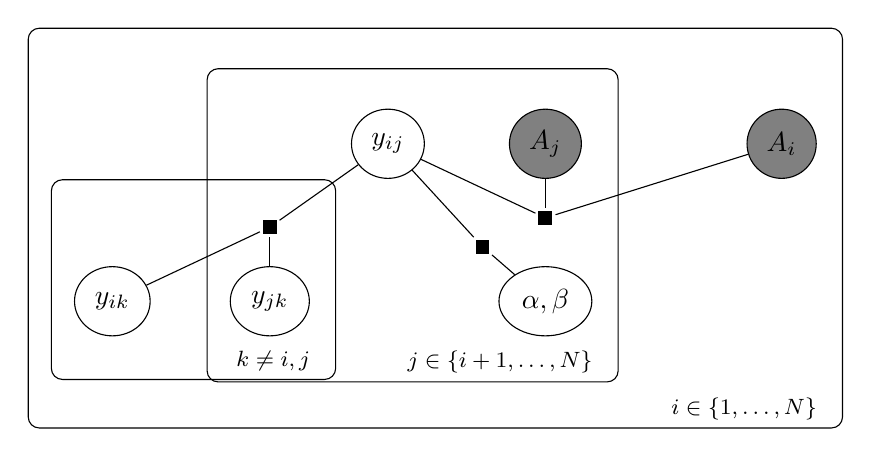
\begin{tikzpicture}[-, >=stealth', shorten >=1pt, auto, node distance=2cm, every state/.style={fill=white, draw=black, text=black, ellipse, align=center}]
	\node[state] (yij) {$y_{ij}$};
	\node[state, fill=gray] (Aj) [right of=yij] {$A_j$};
	\node[state, fill=gray] (Ai) [right of=Aj, xshift=1cm] {$A_i$};
	\node[state] (hyperparams) [below of=Aj] {$\alpha, \beta$};
	\node[state] (yjk) [below of=yij, xshift=-1.5cm] {$y_{jk}$};
	\node[state] (yik) [left of=yjk] {$y_{ik}$};
	\factor[below =of Aj] {appearance-f} {} {} {};
	\factor[above left=of hyperparams] {hp-f} {} {} {};
	\factor[above=of yjk] {edge-f} {} {} {};
	
	\factoredge {yij} {appearance-f} {} ;
	\factoredge {Ai} {appearance-f} {} ;
	\factoredge {Aj} {appearance-f} {} ;
	\factoredge {hyperparams} {hp-f} {} ;
	\factoredge {yij} {hp-f} {} ;
	\factoredge {yij} {edge-f} {} ;
	\factoredge {yjk} {edge-f} {} ;
	\factoredge {yik} {edge-f} {} ;
		
	\plate [inner sep=.3cm,xshift=.02cm,yshift=.2cm] {platek} {(yik)(yjk)(edge-f)} {$k \neq i, j$};
	\plate [inner sep=.3cm,xshift=.02cm,yshift=.2cm] {platej} {(yij)(Aj)(hyperparams)(yjk)} {$j \in \{i+1, \ldots, N\}$};
	\plate [inner sep=.3cm,xshift=.02cm,yshift=.2cm] {platei} {(Ai)(yik)(platej)(platek)} {$i \in \{1, \ldots, N\}$};
\end{tikzpicture}
\caption{Potential graphical model with multiple additions. $y_{ij}, y_{jk}, y_{ik}$ have factor increasing the probability of the third if the other two equal 1. $\alpha, \beta$ are hyperparameters on a prior on the distribution of $y_{ij}$.}
\label{fig:model}
\end{figure}

\section{Challenges}
There are two challenges to overcome. First, we must learn feature functions $\phi$ for the probability of $y_{ij}$ given $A_i, A_j$ and for the joint distribution $p(y_{ij}, y_{jk}, y_{ik})$. We can obtain the true graph structures of proteins using data from the Protein Data Bank, then use these graph structures, along with the corresponding amino acid sequences, to determine these distributions. We are also looking into using evolutionary data to determine if certain types of amino acids are more or less likely to interact. Second, we must perform inference on the graphical model. This may be possible using loopy belief propagation (although with the additional factor $p(y_{ij}, y_{jk}, y_{ik})$ the graph will be very loopy).

%Additionally, we hope to further refine the estimated structure using D-PMP inference. We plan to initialize inference using the estimated (potentially flawed) graph structure. Then, after performing inference for some number of iterations, we will use the result to obtain a new graph structure. It is unlikely that inference will find the exact positions of amino acids using a flawed graph structure, however it may be able to find approximate positions and thus fix missing links or remove unnecessary ones in the graph structure.

\section{Data}
	To train and test our model, we are using protein data from the Protein Data Bank. PDB files contain x, y, z coordinates for each atom in each amino amino acid of a protein. From these coordinates, distances between atoms can be computed and converted into a graph, where edges exist between amino acids if they lie within a threshold distance $d$ of each other, with $d = 10 {\AA}$ for our initial data processing. We are using a 1000-protein set for our initial model training and testing, with 750 allocated for training and 250 for test. These graphs will serve two primary purposes: training and testing our factor potentials, as well as providing ground-truth data for our edge prediction model. Fig. \ref{fig:contactgraph} contains example of a graph produced from a processed PBD file. 

\begin{figure}
\centering
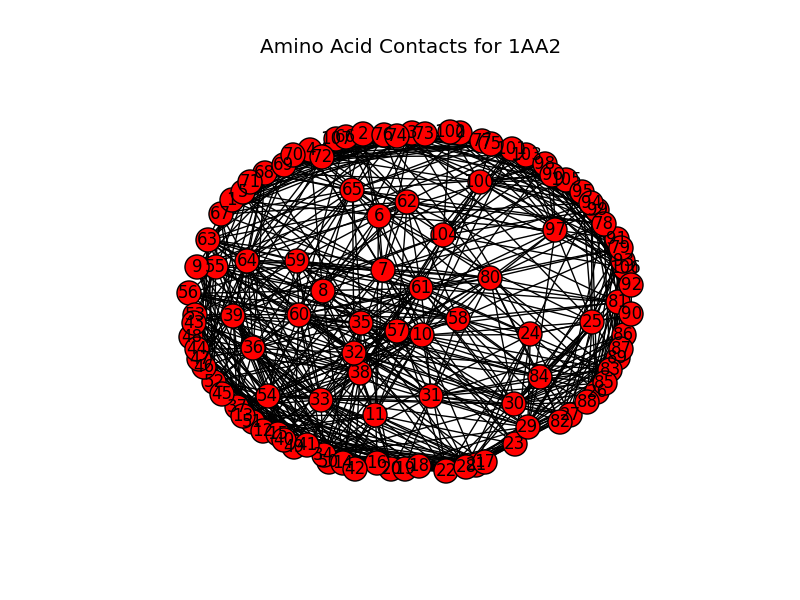
\includegraphics[scale=0.3]{1aa2_plot.png}
\caption{Amino Acid Contact graph for Protein 1AA2.}
\label{fig:contactgraph}
\end{figure}
 
We observe that for this protein, most edges are highly localized among adjacent amino acids. However, many edges have connections across the protein, which is in and of itself an indicator of protein fold structure. We also observe that this graph is relatively sparse (compared to the complete graph), with 882 edges connecting 108 amino acids. 


\section{Evaluation}
As mentioned above, methods for protein contact prediction already exist, at least two of which are freely available on the internet\cite{ekeberg13} \cite{wang16}. The CoinFold model described by Wang et al. uses both the amino acid sequence and evolutionary data to predict contact between amino acids in a protein. It is not a direct parallel, because CoinFold attempts to minimize total error, while we seek to minimize false negatives. Despite this, CoinFold would likely provide a good baseline against which to evaluate. The Ekeberg et al. \cite{ekeberg13} Potts model could also provide a valuable baseline for our model. A key concept used in the evaluation of both systems is the difference between short, medium, and long-range contacts. Predicting contacts between amino acids that are close in the sequence is intuitively simpler than predicting long-range contacts, which may implicitly represent complex secondary and tertiary protein structure. 

We also plan to evaluate different models against each other. For example, the model with joint $p(y_{ij}, y_{jk}, y_{ik})$ can be evaluated against the naive model involving only unary factors (assuming $A_i, A_j$ are observed). To evaluate the use of our model combined with D-PMP inference, we plan to initialize D-PMP inference with different graph structures including a complete graph, a random graph, and a graph with connections only along the backbone (i.e. between amino acids $A_i$ and $A_{i+1}$). This will help determine what improvements come from our model versus from D-PMP inference. 

\section{Timeline}
\textbf{Week 1:} Create features based on distance in amino acid sequence and amino acid type. Implement and test simple model. Run on CoinFold and other benchmarks.
\textbf{Week 2:} Experiment with different models (e.g. factors between triplets of edge indicator variables). Experiment with adding priors to the models.
\textbf{Week 3:} Look into contextual feature functions (take into account surrounding amino acids). Look into evolutionary-based feature functions
\textbf{Week 4:} Preliminary evaluation (750 training, 250 test proteins). Create presentation.
\textbf{Week 5-6:} Experiment with iterative improvement via DPMP. Stretch goal: use secondary structure prediction to estimate contacts. Stretch goal: use CryoEM data to predict contacts. Write paper.

\begin{thebibliography}{9}
{\setlength\itemsep{0.0em}
\bibitem{wuyun16}
	Qiqige Wuyun, Wei Zheng, Zhenling Peng, and Jianyi Yang. November 1, 2016. A large-scale comparative assessment of methods for residue?residue contact prediction. Brief Bioinform (2016) doi:10.1093/bib/bbw106
\bibitem{colwell11}
	Debora S. Marks, Lucy J. Colwell, Robert Sheridan, Thomas A. Hopf, Andrea Pagnani, Riccardo Zecchina, Chris Sander. 25 October 2011. 3D Protein Structure Predicted from Sequence. {\tt arXiv:1110.5091 [q-bio.BM]}
\bibitem{ekeberg13}
	Magnus Ekeberg, Cecilia L{\"o}vkvist, Yueheng Lan, Martin Weigt, Erik Aurell. 12 January 2013. Improved contact prediction in proteins: Using pseudolikelihoods to infer Potts models. {\tt arXiv:1211.1281 [q-bio.QM]}
\bibitem{ma15}
	 Ma J., Wang S., Wang Z., Xu J. August 14, 2015. Protein contact prediction by integrating joint evolutionary coupling analysis and supervised learning. Bioinformatics 2015:btv472
\bibitem{wang16}
	Sheng Wang,  Wei Li, Renyu Zhang, Shiwang Liu and Jinbo Xu. April 12, 2016. CoinFold: a web server for protein contact prediction and contact-assisted protein folding. Nucl. Acids Res. (2016) doi: 10.1093/nar/gkw307
\bibitem{golkov16}
	Vladimir Golkov, Marcin J. Skwark, Antonij Golkov, Alexey Dosovitskiy, Thomas Brox, Jens Meiler, and Daniel Cremers. Protein contact prediction from amino acid co-evolution using convolutional networks for graph-valued images. In Proceedings of the 30th Conference on Neural Information Processing Systems (NIPS 2016), Barcelona, Spain.
%\bibitem{pdb}
%	H.M. Berman, J. Westbrook, Z. Feng, G. Gilliland, T.N. Bhat, H. Weissig, I.N. Shindyalov, P.E. Bourne. 2000. The Protein Data Bank
%Nucleic Acids Research, 28: 235-242.
}
\end{thebibliography}

\end{document}